\section{Rule 30: the automorphism group is \texorpdfstring{$\Z^2$}{Z\^{}2}}\label{sec:rigidity30}

Throughout this section $f(a,b,c)=a\oplus(b\vee c)$ is rule $30$ and $F=F_{30}$, so that
\[
F(c)_i=\bigl(y_i,\;x_i\oplus y_{i-1}\oplus(y_i\vee y_{i+1})\bigr).
\]
By Lemma~\ref{lem:spacetime}, $\Aut(X_F)$ is the group of invertible block maps of $\A^{\Z}$ that commute with $F$, and we use this description throughout. We prove that for rule $30$ this group is as small as possible, namely $\langle\sh,F\rangle\cong\Z^2$.

\begin{theorem}\label{thm:rigidity30}
$\Aut(X_{F_{30}})=\langle\sh,F_{30}\rangle$, and $\langle\sh,F_{30}\rangle\cong\Z^2$. More precisely, every invertible block map $h$ with $hF_{30}=F_{30}h$ equals $\sh^aF_{30}^b$ for exactly one $(a,b)\in\Z^2$, namely $a=-\tfrac12(e^+(h)+e^-(h))$ and $b=\tfrac12(e^+(h)-e^-(h))$, where $e^+$ is the forward offset of Theorem~\ref{r30:thm:front}, which does not depend on the radius bound $R$ used to define it, and $e^-(h)=e^+(\rho h\rho)$ is the backward offset of Corollary~\ref{r30:cor:offsets}.
\end{theorem}

In particular $F_{30}$ has infinite order, and $\sh^aF_{30}^b=\mathrm{id}$ only for $a=b=0$; this part is elementary, since by Lemma~\ref{r30:lem:transl} the map $\sh^aF^b$ shifts the forward intercept of every pair by $b-a$ and the backward intercept by $-a-b$; applied to a single $y$-flip, whose intercepts are both finite, this shows that $\sh^aF^b$ moves them unless $a=b=0$. The theorem concerns automorphisms. The endomorphism monoid $\Cent(F_{30})$ contains the two constant maps onto the fixed points $(0,0)^{\Z}$ and $(1,1)^{\Z}$ (Section~\ref{sec:prelim}), and we do not determine it: the proof below uses the invertibility of $h$ in an essential way (Lemma~\ref{r30:lem:onset}).

\medskip
\noindent\textbf{Strategy.} We work with pairs of configurations that agree far to the right, and with the rightmost difference $\lambda_t$ in row $t$ of their spacetime diagrams. Because rule $30$ is permutive in its left argument and the second-order rule is permutive in the previous row, the rightmost difference moves forward in time along a line $i=t+U$ and backward in time along a line $i=V-t$, with at most one exceptional row between them (Proposition~\ref{r30:prop:profile}). We call $U$ and $V$ the forward and backward intercepts of the pair. The main step (Theorem~\ref{r30:thm:front}) is that an automorphism $h$ shifts the forward intercept of every \emph{front pair} (a pair whose rightmost difference is a $y$-bit) by the same integer $e^+(h)$. The shift $E(P)$ is a function of a finite window of the pair, and it is unchanged when the pair is advanced by $F$ (Lemma~\ref{r30:lem:E}). Let $e_{\max}$ be its largest value. A maximum principle (Lemma~\ref{r30:lem:max}) shows that the pairs with $E=e_{\max}$ stay so under arbitrary changes behind the front, so whether $E(P)=e_{\max}$ depends only on the cells of one configuration at and just ahead of the front (Corollary~\ref{r30:cor:word}). The set of words with this property is nonempty and forward-closed in a finite graph $\Lambda_M$ that follows one configuration along the light-speed front, and $\Lambda_M$ is strongly connected (Lemma~\ref{r30:lem:lambda}), so the set contains every word and the shift is constant. The graph $\Lambda_M$ is built as a tower of factor graphs in which each layer adds one bit, and the lifting step uses a closed walk along which the new bit changes an odd number of times; for rule $30$ this walk is a single loop. Constancy extends from front pairs to all pairs (Lemma~\ref{r30:lem:allpairs}), and through the time reversal $\rho(x,y)=(y,x)$ to the backward intercept. This gives a homomorphism $(e^+,e^-)\colon\Aut(X_F)\to\Z^2$ that is injective on $\langle\sh,F\rangle$. If $e^+(h)=e^-(h)=0$, then the value of $h$ at a point of spacetime depends only on the right light cone of that point (Proposition~\ref{r30:prop:cone}). It is permutive in both edges of the cone (Proposition~\ref{r30:prop:edges}), hence equals the identity plus a correction that depends only on the part of the cone strictly to the right of the apex, and the commutation relation forces the correction to vanish (Lemma~\ref{r30:lem:gamma}). Finally, a parity argument on the four spatially constant configurations shows that $e^+\equiv e^-\pmod 2$ (Lemma~\ref{r30:lem:parity}), so every automorphism is brought to offsets $(0,0)$ by an element of $\langle\sh,F\rangle$. Figure~\ref{r30:fig:profile} shows the profile of a pair, and Figure~\ref{r30:fig:cone} the light cone.

\medskip
\noindent\textbf{Conventions.} Bits are combined with $\oplus$, $\vee$, $\wedge$ and $\neg$. For a statement $S$, $[S]\in\{0,1\}$ is $1$ if $S$ holds and $0$ otherwise. Intervals $[m,n]$ are intervals of integers. We use $-\infty$ with the conventions $-\infty+k=-\infty<n$ for all integers $k,n$, and $\max\emptyset=-\infty$.

\subsection{Diagrams, pairs and profiles}\label{r30:sec:diagrams}

For $c\in\A^{\Z}$ and $t\in\Z$ let $y^t\in\{0,1\}^{\Z}$ be the $y$-row of $F^t(c)$. The $x$-row of $F(d)$ is the $y$-row of $d$, so the $x$-row of $F^t(c)$ is $y^{t-1}$, and in particular $c_i=(y^{-1}_i,y^0_i)$. The \emph{diagram} of $c$ is $Y_c\colon\Z^2\to\{0,1\}$, $Y_c(t,i)=y^t_i$. By \eqref{eq:F}, every diagram satisfies
\begin{equation}\label{r30:eq:rec}
Y(t+1,i)\oplus Y(t-1,i)\oplus Y(t,i-1)=Y(t,i)\vee Y(t,i+1)\qquad\text{for all }(t,i)\in\Z^2.
\end{equation}
The relation is an exclusive or in each of $Y(t+1,i)$, $Y(t-1,i)$ and $Y(t,i-1)$, so each of these three values is determined by the other four. Using the first two, any two consecutive rows determine all rows. Hence $c\mapsto Y_c$ is a bijection from $\A^{\Z}$ onto the set of solutions of \eqref{r30:eq:rec}, and two diagrams that agree on two consecutive rows are equal. Translations act by
\begin{equation}\label{r30:eq:transl}
Y_{\sh^jF^kc}(t,i)=Y_c(t+k,\,i+j).
\end{equation}
If $h$ is a block map commuting with $F$, then $F^th(c)=h(F^tc)$, so
\begin{equation}\label{r30:eq:rows}
\text{rows $t-1$ and $t$ of $Y_{hc}$ are the $x$-row and the $y$-row of $h(F^tc)$.}
\end{equation}

\paragraph{Time reversal.} Let $\rho\colon\A^{\Z}\to\A^{\Z}$ exchange the two bits of every cell, $\rho(c)_i=(y_i,x_i)$. That this exchange reverses time is noted in \cite[p.~2500]{Takesue1987}. From \eqref{eq:F}, $F(\rho c)_i=\bigl(x_i,\;y_i\oplus f(x_{i-1},x_i,x_{i+1})\bigr)$, so $\rho F\rho(c)_i=\bigl(y_i\oplus f(x_{i-1},x_i,x_{i+1}),\,x_i\bigr)=F^{-1}(c)_i$ by \eqref{eq:Finv}. Thus $\rho F\rho=F^{-1}$, and clearly $\rho\sh=\sh\rho$. Consequently $\rho h\rho$ is an invertible block map commuting with $F$ whenever $h$ is, and $h\mapsto\rho h\rho$ is an automorphism of the group $\Aut(X_F)$. Since $F^t\rho=\rho F^{-t}$ and the $y$-row of $\rho d$ is the $x$-row of $d$,
\begin{equation}\label{r30:eq:rho}
Y_{\rho c}(t,i)=Y_c(-1-t,\,i).
\end{equation}

\paragraph{Pairs and profiles.} A \emph{pair} is an ordered pair $Q=(c,c')$ of distinct configurations with $c_i=c'_i$ for all sufficiently large $i$. Its difference diagram is $\Delta_Q=Y_c\oplus Y_{c'}$. If $h$ is an invertible block map commuting with $F$, then $hQ=(hc,hc')$ is again a pair ($hc\ne hc'$ because $h$ is injective, and if $c,c'$ agree to the right of $s$ and $h$ has radius $R$, then $hc,hc'$ agree to the right of $s+R$), and so are $F^kQ$, $\sh^jQ$ and $\rho Q$, defined componentwise.

If rows $t-1$ and $t$ of $\Delta_Q$ vanish to the right of a site $s$, then by \eqref{r30:eq:rec} rows $t+1$ and $t-2$ vanish to the right of $s+1$. Rows $-1$ and $0$ vanish far to the right by definition, so by induction every row of $\Delta_Q$ does. The \emph{profile} of $Q$ is
\[
\lambda_t=\lambda_t(Q)=\max\{i:\Delta_Q(t,i)=1\}\in\Z\cup\{-\infty\}\qquad(t\in\Z).
\]

\begin{lemma}\label{r30:lem:R}
For every pair and every $t\in\Z$:
\begin{enumerate}
\item $\lambda_{t+1}\le\max(\lambda_{t-1},\lambda_t+1)$, with equality if $\lambda_{t-1}\ne\lambda_t+1$;
\item $\lambda_{t-1}\le\max(\lambda_{t+1},\lambda_t+1)$, with equality if $\lambda_{t+1}\ne\lambda_t+1$.
\end{enumerate}
\end{lemma}

\begin{proof}
By \eqref{r30:eq:rec},
\[
\Delta(t+1,i)=\Delta(t-1,i)\oplus\Delta(t,i-1)\oplus\bigl[(Y_c(t,i)\vee Y_c(t,i+1))\oplus(Y_{c'}(t,i)\vee Y_{c'}(t,i+1))\bigr].
\]
Let $m=\max(\lambda_{t-1},\lambda_t+1)$. For $i>m$ all three terms vanish, the last because $i,i+1>\lambda_t$. Suppose $m$ is finite. At $i=m$ the last term vanishes for the same reason. Since $m\ge\lambda_{t-1}$ and $m-1\ge\lambda_t$, we have $\Delta(t-1,m)=[m=\lambda_{t-1}]$ and $\Delta(t,m-1)=[m-1=\lambda_t]$. At least one of these is $1$, because $m$ is one of $\lambda_{t-1},\lambda_t+1$, and both are $1$ only if $\lambda_{t-1}=\lambda_t+1$. So $\Delta(t+1,m)=1$ when $\lambda_{t-1}\ne\lambda_t+1$. This proves (1). Part (2) is the same argument applied to \eqref{r30:eq:rec} solved for $Y(t-1,i)$, which has the same form with $t+1$ and $t-1$ exchanged.
\end{proof}

\begin{proposition}\label{r30:prop:profile}
Let $Q$ be a pair with profile $\lambda_t$, and put
\[
I^+=\{t:\lambda_t\ne-\infty,\ \lambda_t\ge\lambda_{t-1}\},\qquad I^-=\{t:\lambda_t\ne-\infty,\ \lambda_t\ge\lambda_{t+1}\}.
\]
\begin{enumerate}
\item No two consecutive $\lambda_t$ equal $-\infty$.
\item If $t\in I^+$, then $t+1\in I^+$ and $\lambda_{t+1}=\lambda_t+1$. If $t\in I^-$, then $t-1\in I^-$ and $\lambda_{t-1}=\lambda_t+1$. The sets $I^+$ and $I^-$ are disjoint, and every element of $I^-$ is smaller than every element of $I^+$.
\item The set $\Z\setminus(I^+\cup I^-)$ has at most one element. If $m$ is such an element (a \emph{middle row}), then $m-1\in I^-$, $m+1\in I^+$ and $\lambda_m<\lambda_{m-1}=\lambda_{m+1}$. If $I^+=\emptyset$ then $I^-=\Z$, and if $I^-=\emptyset$ then $I^+=\Z$.
\item Define the \emph{forward intercept} $U=U(Q)$ and the \emph{backward intercept} $V=V(Q)$ by $U=\lambda_t-t$ for $t\in I^+$ and $V=\lambda_t+t$ for $t\in I^-$ (well defined by (2)), with $U=-\infty$ if $I^+=\emptyset$ and $V=-\infty$ if $I^-=\emptyset$. Then $\lambda_t\le\max(t+U,\,V-t)$ for all $t$. Equivalently, $\Delta_Q(t,i)=1$ implies $i-t\le U$ or $i+t\le V$.
\item Suppose $U$ and $V$ are finite. If $V-U$ is odd, there is no middle row, and $I^+=[t_+,\infty)$, $I^-=(-\infty,t_+-1]$ with $2t_+-1=V-U$. If $V-U$ is even, there is a middle row $m=(V-U)/2$, and $I^+=[m+1,\infty)$, $I^-=(-\infty,m-1]$.
\item For every $t$, $U\le\max(\lambda_t-t,\ \lambda_{t-1}-t-1)$ and $V\le\max(\lambda_t+t,\ \lambda_{t+1}+t-1)$.
\end{enumerate}
\end{proposition}

\begin{figure}[ht]
\centering
\begin{tikzpicture}[x=0.5cm,y=0.5cm,font=\small]
\foreach \t/\l in {-2/6,-1/5,0/4,1/3,2/1,3/3,4/4,5/5,6/6}{
  \fill[black!12] (-3,\t-0.4) rectangle (\l+0.4,\t+0.4);
  \fill (\l,\t) circle (0.18);
}
\draw[thick] (3,3) -- (6.7,6.7) node[right] {$i=t+U$};
\draw[thick] (3,1) -- (6.7,-2.7) node[right] {$i=V-t$};
\draw[dashed] (3,3) -- (2,2) -- (3,1);
\draw[-{Stealth[length=2mm]}] (-3.6,-3) -- (-3.6,7.2) node[above] {$t$};
\draw[-{Stealth[length=2mm]}] (-3.6,-3) -- (8.5,-3) node[right] {$i$};
\node[right] at (9.3,4.5) {$I^+$:\ \ $\lambda_t=t+U$};
\node[right] at (9.3,2) {middle row $m$:\ \ $\lambda_m<\lambda_{m\pm1}$};
\node[right] at (9.3,-0.5) {$I^-$:\ \ $\lambda_t=V-t$};
\draw[black!50] (9.2,2) -- (1.6,2);
\end{tikzpicture}
\caption{The profile of a pair with $U$, $V$ finite and $V-U$ even (Proposition~\ref{r30:prop:profile}). Each row $t$ of the difference diagram vanishes outside the shaded sites $i\le\lambda_t$, and the dot marks the rightmost difference $\lambda_t$. It moves along the line $i=t+U$ for $t\in I^+$ and along $i=V-t$ for $t\in I^-$; the two lines meet in the middle row $m=(V-U)/2$. If $V-U$ is odd there is no middle row.}
\label{r30:fig:profile}
\end{figure}

\begin{proof}
(1) If $\lambda_t=\lambda_{t+1}=-\infty$, then $Y_c$ and $Y_{c'}$ agree on two consecutive rows, so $c=c'$, which is excluded.

(2) If $t\in I^+$ then $\lambda_{t-1}\le\lambda_t<\lambda_t+1$, so Lemma~\ref{r30:lem:R}(1) gives $\lambda_{t+1}=\max(\lambda_{t-1},\lambda_t+1)=\lambda_t+1$; in particular $\lambda_{t+1}\ge\lambda_t$, so $t+1\in I^+$. The statement for $I^-$ follows in the same way from Lemma~\ref{r30:lem:R}(2). If $t\in I^+$ then $\lambda_{t+1}>\lambda_t$, so $t\notin I^-$. If $a\in I^+$ and $b\in I^-$ with $a\le b$, then $b\in I^+$ by the first statement, contradicting disjointness.

(3) Let $t\notin I^+\cup I^-$. If $\lambda_t=-\infty$, then $\lambda_{t\pm1}$ are finite by (1), and $\lambda_{t+1}\ge\lambda_t$, $\lambda_{t-1}\ge\lambda_t$ give $t+1\in I^+$, $t-1\in I^-$. If $\lambda_t$ is finite, then $t\notin I^+$ gives $\lambda_{t-1}>\lambda_t$ (in particular $\lambda_{t-1}$ is finite), so $t-1\in I^-$; and $t\notin I^-$ gives $\lambda_{t+1}>\lambda_t$, so $t+1\in I^+$. If $t<t'$ were two such elements, then $t+1\in I^+$ and (2) would give $t'\in I^+$. Hence there is at most one. If $I^+=\emptyset$, no such element can exist (it would have $t+1\in I^+$), so $I^-=\Z$; symmetrically for $I^-=\emptyset$.

Now let $m$ be a middle row; we have shown $m\pm1\in I^\pm$ and $\lambda_m<\lambda_{m\pm1}$. If $\lambda_m=-\infty$, then $\lambda_{m-1}\ne\lambda_m+1$ and Lemma~\ref{r30:lem:R}(1) gives $\lambda_{m+1}=\lambda_{m-1}$. If $\lambda_m$ is finite and $\lambda_{m-1}\ne\lambda_m+1$, then Lemma~\ref{r30:lem:R}(1) gives $\lambda_{m+1}=\max(\lambda_{m-1},\lambda_m+1)=\lambda_{m-1}$, since $\lambda_{m-1}\ge\lambda_m+1$. If $\lambda_{m-1}=\lambda_m+1$, then $\lambda_{m+1}\le\lambda_m+1$ by Lemma~\ref{r30:lem:R}(1), and $\lambda_{m+1}>\lambda_m$, so $\lambda_{m+1}=\lambda_m+1=\lambda_{m-1}$.

(4) For $t\in I^+$ we have $\lambda_t=t+U$ and for $t\in I^-$ we have $\lambda_t=V-t$. For a middle row $m$, $\lambda_m<\lambda_{m-1}=V-m+1$, so $\lambda_m\le V-m$.

(5) Both $I^+$ and $I^-$ are nonempty. By (2) and (3), $\Z$ is the disjoint union of an interval $I^-=(-\infty,t_-]$, at most one middle row, and an interval $I^+=[t_+,\infty)$. If there is no middle row, then $t_-=t_+-1$; now $t_+\in I^+$ gives $t_++U\ge\lambda_{t_+-1}=V-t_++1$, and $t_+-1\in I^-$ gives $V-t_++1\ge t_++U$, so $V-U=2t_+-1$. If there is a middle row $m$, then $\lambda_{m+1}=\lambda_{m-1}$ reads $m+1+U=V-m+1$, so $V-U=2m$. The two cases give different parities of $V-U$, so the parity decides which case occurs.

(6) Put $\mu_t=\max(\lambda_t-t,\ \lambda_{t-1}-t-1)$. By Lemma~\ref{r30:lem:R}(1), $\lambda_{t+1}-(t+1)\le\max(\lambda_{t-1}-t-1,\ \lambda_t-t)\le\mu_t$, and $\lambda_t-t-2<\lambda_t-t\le\mu_t$, so $\mu_{t+1}\le\mu_t$. If $I^+\ne\emptyset$, then for $t-1\in I^+$ we have $\mu_t=\max(U,U-2)=U$. As $\mu$ is nonincreasing, $U\le\mu_t$ for every $t$; if $I^+=\emptyset$ there is nothing to prove. Similarly $\nu_t=\max(\lambda_t+t,\ \lambda_{t+1}+t-1)$ is nondecreasing by Lemma~\ref{r30:lem:R}(2), and $\nu_t=V$ whenever $t+1\in I^-$; hence $V\le\nu_t$ for every $t$.
\end{proof}

\begin{lemma}\label{r30:lem:transl}
For every pair $Q$ and all $j,k\in\Z$:
$U(F^kQ)=U(Q)+k$ and $V(F^kQ)=V(Q)-k$;
$U(\sh^jQ)=U(Q)-j$ and $V(\sh^jQ)=V(Q)-j$;
$U(\rho Q)=V(Q)+1$ and $V(\rho Q)=U(Q)-1$.
\end{lemma}

\begin{proof}
By \eqref{r30:eq:transl}, $\lambda_t(F^kQ)=\lambda_{t+k}(Q)$ and $\lambda_t(\sh^jQ)=\lambda_t(Q)-j$. So $I^\pm(F^kQ)=I^\pm(Q)-k$, $I^\pm(\sh^jQ)=I^\pm(Q)$, and the formulas for $F^k$ and $\sh^j$ follow. By \eqref{r30:eq:rho}, $\lambda_t(\rho Q)=\lambda_{-1-t}(Q)$. Hence $t\in I^+(\rho Q)$ if and only if $-1-t\in I^-(Q)$, and then $\lambda_t(\rho Q)=V(Q)-(-1-t)=t+V(Q)+1$; and $t\in I^-(\rho Q)$ if and only if $-1-t\in I^+(Q)$, and then $\lambda_t(\rho Q)=(-1-t)+U(Q)=U(Q)-1-t$. The values $-\infty$ correspond to empty sets on both sides.
\end{proof}

\begin{definition}\label{r30:def:front}
A pair $(c,c')$ is a \emph{front pair at $p$} if $c_i=c'_i$ for all $i>p$, $y(c_p)\ne y(c'_p)$ and $x(c_p)=x(c'_p)$; equivalently, $\lambda_0=p>\lambda_{-1}$. For $c\in\A^{\Z}$ and $j\in\Z$, the \emph{$y$-flip}, \emph{$x$-flip} and \emph{$yx$-flip at $j$} are the pairs $(c,c')$ in which $c'$ is obtained from $c$ by complementing, respectively, the bit $y(c_j)$; the bit $x(c_j)$; both bits $y(c_j)$ and $x(c_{j+1})$.
\end{definition}

\begin{lemma}\label{r30:lem:flips}
\begin{enumerate}
\item If $Q$ is a front pair at $p$, then $U(Q)=p$, and $F^tQ$ is a front pair at $p+t$ for every $t\ge0$.
\item A $y$-flip at $j$ is a front pair at $j$, with $(U,V)=(j,j-2)$.
\item If $Q$ is an $x$-flip at $j$, then $FQ$ is a front pair at $j$, and $(U,V)=(j-1,j-1)$.
\item A $yx$-flip at $j$ has $V=j$, and either $U=-\infty$ or $U\le j-1$.
\end{enumerate}
\end{lemma}

\begin{proof}
(1) Here $0\in I^+$, so $U=\lambda_0=p$, and by Proposition~\ref{r30:prop:profile}(2), $\lambda_t=p+t>\lambda_{t-1}$ for all $t\ge0$. Since $\lambda_0(F^tQ)=\lambda_t$ and $\lambda_{-1}(F^tQ)=\lambda_{t-1}$, this says that $F^tQ$ is a front pair at $p+t$.

(2) Here $\lambda_0=j$ and $\lambda_{-1}=-\infty$, so the pair is a front pair at $j$ and $U=j$ by (1). By Lemma~\ref{r30:lem:R}(2) at $t=-1$, since $\lambda_0\ne\lambda_{-1}+1$, $\lambda_{-2}=\max(\lambda_0,\lambda_{-1}+1)=j$. Thus $-2\in I^-$ and $V=j-2$.

(3) Here $\lambda_{-1}=j$ and $\lambda_0=-\infty$. By Lemma~\ref{r30:lem:R}(1) at $t=0$, $\lambda_1=\max(j,-\infty)=j$. So $\lambda_0(FQ)=j>\lambda_{-1}(FQ)=-\infty$, $FQ$ is a front pair at $j$, $1\in I^+$ and $U=j-1$. Also $-1\in I^-$ because $\lambda_{-1}\ge\lambda_0$, so $V=j-1$.

(4) Here $\lambda_0=j$ and $\lambda_{-1}=j+1$, so $-1\in I^-$ and $V=j$. By Lemma~\ref{r30:lem:R}(1), $\lambda_1\le j+1$, and by \eqref{r30:eq:rec}, $\Delta(1,j+1)=\Delta(-1,j+1)\oplus\Delta(0,j)\oplus0=1\oplus1=0$, the last term vanishing because row $0$ of $\Delta$ vanishes at $j+1$ and $j+2$. So $\lambda_1\le j$, and Proposition~\ref{r30:prop:profile}(6) at $t=1$ gives $U\le\max(\lambda_1-1,\lambda_0-2)\le j-1$.
\end{proof}

\subsection{The light-speed window graph}\label{r30:sec:window}

Fix $M\ge0$. Let $\Lambda_M$ be the directed graph whose vertices are the words $\omega=\omega_0\cdots\omega_M\in\A^{M+1}$, with an edge $\omega\to\omega\cdot\iota$ for every $\iota=(\iota_1,\iota_2)\in\A^2$, where
\[
(\omega\cdot\iota)_k=F(\tilde c)_{p+1+k}\qquad(0\le k\le M)
\]
and $\tilde c$ is any configuration with $\tilde c_{p+k}=\omega_k$ for $0\le k\le M$, $\tilde c_{p+M+1}=\iota_1$ and $\tilde c_{p+M+2}=\iota_2$. Since $F$ has radius $1$, the cells $F(\tilde c)_i$ with $p+1\le i\le p+M+1$ read only $\tilde c$ on $[p,p+M+2]$, so $\omega\cdot\iota$ depends neither on $p$ nor on the other cells of $\tilde c$. A vertex of $\Lambda_M$ is the word of a single configuration on a cell $p$ (the \emph{front}) and the $M$ cells ahead of it, and an edge advances the front by one site, at the speed of light.

\begin{lemma}\label{r30:lem:lambda}
For every $M\ge0$, the graph $\Lambda_M$ is strongly connected.
\end{lemma}

The proof occupies the rest of this subsection. It builds $\Lambda_M$ as a tower of $2M+2$ factor graphs, each of which adds one bit to the previous one (Figure~\ref{r30:fig:layers}).

\paragraph{Layer coordinates.} For a vertex $\omega$ of $\Lambda_M$, placed on the sites $[p,p+M]$, put
\begin{equation}\label{r30:eq:layers}
y[d]=y(\omega_{-d})\ \ (-M\le d\le0),\qquad x[k]=x(\omega_{-k-1})\ \ (-M-1\le k\le-1).
\end{equation}
Thus the cell at site $p-d$ is $(x[d-1],y[d])$, and a vertex is the same as an arbitrary assignment of bits to the $2M+2$ \emph{layers} $y[-M],\dots,y[0]$ and $x[-M-1],\dots,x[-1]$. The index of a layer is a comoving coordinate: if $c$ is a configuration and $z_t[d]$ denotes the $y$-bit of $F^t(c)$ at site $p+t-d$, then the word of $F^t(c)$ on $[p+t,p+t+M]$ has $y$-layers $z_t[d]$ and $x$-layers $z_{t-1}[k]$.

\begin{figure}[ht]
\centering
\begin{tikzpicture}[x=1.55cm,y=0.62cm,font=\small]
\foreach \j/\d in {0/0,1/-1,2/-2,3/-3}{
  \draw (\j,0) rectangle (\j+1,1);
  \draw (\j,1) rectangle (\j+1,2);
}
\node at (0.5,1.5) {$x[-1]$}; \node at (0.5,0.5) {$y[0]$};
\node at (1.5,1.5) {$x[-2]$}; \node at (1.5,0.5) {$y[-1]$};
\node at (2.5,1.5) {$x[-3]$}; \node at (2.5,0.5) {$y[-2]$};
\node at (3.5,1.5) {$x[-4]$}; \node at (3.5,0.5) {$y[-3]$};
\node[above] at (0.5,2) {$p$}; \node[above] at (1.5,2) {$p+1$}; \node[above] at (2.5,2) {$p+2$}; \node[above] at (3.5,2) {$p+3$};
\node[left] at (0,1.5) {$x$-bit}; \node[left] at (0,0.5) {$y$-bit};
\foreach \j/\a/\b in {0/7/8,1/5/6,2/3/4,3/1/2}{
  \node[font=\scriptsize,text=black!60] at (\j+0.86,1.2) {\a};
  \node[font=\scriptsize,text=black!60] at (\j+0.86,0.2) {\b};
}
\draw[dashed] (4,0) rectangle (5,2); \draw[dashed] (5,0) rectangle (6,2);
\node at (4.5,1) {$\iota_1$}; \node at (5.5,1) {$\iota_2$};
\node[above] at (4.5,2) {$p+4$}; \node[above] at (5.5,2) {$p+5$};
\draw[-{Stealth[length=2mm]}] (0.5,-0.5) -- node[below] {front moves one site per step} (1.5,-0.5);
\end{tikzpicture}
\caption{A vertex of $\Lambda_M$ for $M=3$, with its layer coordinates \eqref{r30:eq:layers} and the two input cells $\iota_1,\iota_2$ of an edge. The small numbers give the order $L_1,\dots,L_8$ in which the tower adds the layers: from the cell farthest ahead of the front back to the front, and within a cell first the $x$-bit, then the $y$-bit.}
\label{r30:fig:layers}
\end{figure}

\begin{lemma}[layer equation]\label{r30:lem:layer}
Let $\omega$ be a vertex of $\Lambda_M$ and $\iota=(\iota_1,\iota_2)\in\A^2$, let $y',x'$ be the layers of $\omega'=\omega\cdot\iota$, and put
\[
u=y(\iota_1),\qquad v=x(\iota_1)\oplus y(\omega_M)\oplus\bigl(y(\iota_1)\vee y(\iota_2)\bigr).
\]
Then:
\begin{enumerate}
\item $x'[-M-1]=u$, and $x'[k]=y[k]$ for $-M\le k\le-1$;
\item $y'[-M]=v$;
\item for $-M+1\le d\le0$,
\begin{equation}\label{r30:eq:L}
y'[d]=y[d]\oplus x[d-2]\oplus\bigl(y[d-1]\vee y[d-2]\bigr),
\end{equation}
with the convention $y[-M-1]=u$.
\end{enumerate}
The map $\iota\mapsto(u,v)$ is onto $\{0,1\}^2$. So every vertex $\omega$ has exactly four successors, the vertices $\omega\cdot(u,v)$, $(u,v)\in\{0,1\}^2$, given by \textup{(1)--(3)}.
\end{lemma}

\begin{proof}
Let $\tilde c$ be as in the definition of $\omega\cdot\iota$. The new cell at a site $i$ is $F(\tilde c)_i=\bigl(y(\tilde c_i),\,x(\tilde c_i)\oplus y(\tilde c_{i-1})\oplus(y(\tilde c_i)\vee y(\tilde c_{i+1}))\bigr)$, and the layers of $\omega'$ are taken with respect to the new front $p+1$. So $x'[k]$ is the $x$-bit of the new cell at site $p-k$, which is the old $y$-bit at that site: this is $y[k]$ if $p-k\le p+M$, and $y(\iota_1)=u$ if $k=-M-1$. Likewise $y'[d]$ is the $y$-bit of the new cell at site $i=p+1-d$. For $d=-M$ this site is $p+M+1$, and the bit is $v$. For $d\ge-M+1$ we have $i\le p+M$, and $x(\tilde c_i)=x[d-2]$, $y(\tilde c_{i-1})=y[d]$, $y(\tilde c_i)=y[d-1]$ and $y(\tilde c_{i+1})=y[d-2]$, where $y[-M-1]$ stands for the $y$-bit at site $p+M+1$, which is $u$. Given $(u,v)$, take $y(\iota_1)=u$, any $\iota_2$, and $x(\iota_1)=v\oplus y(\omega_M)\oplus(u\vee y(\iota_2))$.
\end{proof}

Equation \eqref{r30:eq:L} is \eqref{r30:eq:rec} written in comoving coordinates. It is lower triangular: $y'[d]$ reads only layers with index at most $d$.

\paragraph{The tower.} Order the $N=2M+2$ layers as
\[
L_1=x[-M-1],\ \ L_2=y[-M],\ \ L_3=x[-M],\ \ L_4=y[-M+1],\ \ \dots,\ \ L_{N-1}=x[-1],\ \ L_N=y[0],
\]
that is, $x[d-1]$ followed by $y[d]$ for $d=-M,\dots,0$. Let $P_n=\{L_1,\dots,L_n\}$, and let $\pi_n$ be the restriction of an assignment of bits to $P_n$. By Lemma~\ref{r30:lem:layer}, the new value of each layer depends only on $(u,v)$ and on layers that precede it or equal it in this order: $x'[k]$ is $u$ or $y[k]$, which precedes $x[k]$; $y'[-M]$ is $v$; and $y'[d]$ reads $y[d]$ and the earlier layers $x[d-2]$, $y[d-1]$ and $y[d-2]$ (or $u$). Hence $\pi_n(\omega\cdot(u,v))$ depends only on $\pi_n(\omega)$ and $(u,v)$. Let $\Lambda^{(n)}$ be the graph with vertex set $\{0,1\}^{P_n}$ and an edge $\eta\to\eta\cdot(u,v):=\pi_n(\omega\cdot(u,v))$, labelled $(u,v)$, for every $\eta$ and $(u,v)$, where $\omega$ is any vertex of $\Lambda_M$ with $\pi_n(\omega)=\eta$. Then:
\begin{itemize}
\item $\Lambda^{(N)}$ has the same vertices and the same successor sets as $\Lambda_M$, so one is strongly connected if and only if the other is;
\item every walk of $\Lambda^{(n)}$ lifts, with the same labels, to a walk of $\Lambda^{(n+1)}$ starting at any vertex that restricts to its initial vertex.
\end{itemize}

\begin{proof}[Proof of Lemma~\ref{r30:lem:lambda}]
We show by induction on $n$ that $\Lambda^{(n)}$ is strongly connected for $2\le n\le N$.

\emph{Base.} The vertices of $\Lambda^{(2)}$ are the values of $(x[-M-1],y[-M])$, and by Lemma~\ref{r30:lem:layer}(1),(2) the edge labelled $(u,v)$ leads from every vertex to $(u,v)$. So $\Lambda^{(2)}$ is a complete digraph with loops.

\emph{Predecessors.} Every vertex $\omega_2$ of $\Lambda_M$, with layers $y_2,x_2$, has an in-neighbour, and every in-neighbour $\hat\omega$ of $\omega_2$, with layers $\hat y,\hat x$, satisfies $\hat y[k]=x_2[k]$ for $-M\le k\le-1$. The second statement is Lemma~\ref{r30:lem:layer}(1). For the first, put $u=x_2[-M-1]$, $v=y_2[-M]$, $\hat y[k]=x_2[k]$ for $-M\le k\le-1$ and $\hat y[0]=0$, and then, with $\hat y[-M-1]=u$,
\[
\hat x[d-2]=y_2[d]\oplus\hat y[d]\oplus\bigl(\hat y[d-1]\vee\hat y[d-2]\bigr)\qquad(-M+1\le d\le0),
\]
and $\hat x[-1]=0$. The indices $d-2$ are distinct and lie in $[-M-1,-2]$, so this defines a vertex $\hat\omega$, and $\hat\omega\cdot(u,v)=\omega_2$ by Lemma~\ref{r30:lem:layer}.

\emph{The step $L_{n+1}=x[k]$, $-M\le k\le-1$.} Assume $\Lambda^{(n)}$ is strongly connected. Write the vertices of $\Lambda^{(n+1)}$ as $(\eta,\chi)$ with $\eta\in\{0,1\}^{P_n}$ and $\chi$ the bit $x[k]$. By Lemma~\ref{r30:lem:layer}, the layer $x[k]$ is read, if at all, only by $y'[k+2]$, which is not in $P_{n+1}$, and its new value is $x'[k]=y[k]$, with $y[k]\in P_n$. So the edge labelled $(u,v)$ goes from $(\eta,\chi)$ to $(\eta\cdot(u,v),\,y[k](\eta))$. Let $(\eta_1,\chi_1)$ and $(\eta_2,\chi_2)$ be vertices of $\Lambda^{(n+1)}$. Extend $(\eta_2,\chi_2)$ to a vertex $\omega_2$ of $\Lambda_M$ and take an in-neighbour $\hat\omega$ of $\omega_2$, with $\hat\omega\cdot(u,v)=\omega_2$. Then $\hat\eta=\pi_n(\hat\omega)$ has an edge labelled $(u,v)$ to $\eta_2$, and $y[k](\hat\eta)=\hat y[k]=x_2[k]=\chi_2$. Take a walk from $\eta_1$ to $\hat\eta$ in $\Lambda^{(n)}$ and lift it to $\Lambda^{(n+1)}$ starting at $(\eta_1,\chi_1)$. It ends at $(\hat\eta,\chi')$ for some $\chi'$, and the edge labelled $(u,v)$ then leads to $(\eta_2,\chi_2)$.

\emph{The step $L_{n+1}=y[d]$, $-M+1\le d\le0$.} Assume $\Lambda^{(n)}$ is strongly connected. Here $P_n$ consists of all layers with index at most $d-1$. For an edge of $\Lambda^{(n)}$ from $\eta$ with label $(u,v)$ put
\[
\phi=x[d-2]\oplus\bigl(y[d-1]\vee y[d-2]\bigr)\in\Z/2,
\]
evaluated on $\eta$, with $y[-M-1]=u$. By \eqref{r30:eq:L}, the edges of $\Lambda^{(n+1)}$ are $(\eta,z)\to(\eta\cdot(u,v),\,z\oplus\phi)$, where $z$ is the bit $y[d]$. The \emph{holonomy} of a walk of $\Lambda^{(n)}$ is the sum in $\Z/2$ of $\phi$ over its edges; the lift of the walk from $(\eta,z)$ ends at a vertex whose last bit is $z$ plus the holonomy.

Let $\eta_*\in\{0,1\}^{P_n}$ be the vertex with
\begin{equation}\label{r30:eq:loop}
y[d-1]=x[d-1]=1,\qquad\text{and all other layers of $P_n$ equal to $0$.}
\end{equation}
We claim that the edge from $\eta_*$ labelled $(u,v)=(0,\,y[-M])$ is a loop, with $\phi=1$. Indeed, by Lemma~\ref{r30:lem:layer}(1), $x'[-M-1]=u=0$ and $x'[k]=y[k]=x[k]$ for $-M\le k\le d-1$, and by (2), $y'[-M]=v=y[-M]$. For $-M+1\le i\le d-1$ the layers $y[i-1]$, $y[i-2]$ and $x[i-2]$ have index at most $d-2$, so they vanish (for $i-2=-M-1$, by $u=0$), and \eqref{r30:eq:L} gives $y'[i]=y[i]$. Finally $\phi=x[d-2]\oplus(y[d-1]\vee y[d-2])=0\oplus(1\vee y[d-2])=1$.

So $\Lambda^{(n)}$ has a closed walk with holonomy $1$, namely this loop. Let $\eta_2$ be any vertex of $\Lambda^{(n)}$, and choose walks $\alpha$ from $\eta_2$ to $\eta_*$ and $\beta$ from $\eta_*$ to $\eta_2$. The closed walks at $\eta_2$ formed by $\alpha$ followed by $\beta$, and by $\alpha$, the loop and $\beta$, have holonomies of different parity. So there are closed walks of both parities at every vertex. Given vertices $(\eta_1,z_1)$ and $(\eta_2,z_2)$ of $\Lambda^{(n+1)}$, take a walk from $\eta_1$ to $\eta_2$ in $\Lambda^{(n)}$ followed by a closed walk at $\eta_2$, chosen so that the total holonomy is $z_1\oplus z_2$. Its lift from $(\eta_1,z_1)$ ends at $(\eta_2,z_2)$.

Every layer $L_{n+1}$ with $n\ge2$ is covered by one of the two steps, so $\Lambda^{(N)}$ is strongly connected, and hence so is $\Lambda_M$.
\end{proof}

The form $a\oplus(b\vee c)$ of rule $30$ enters this proof only through the loop at $\eta_*$: it is a stationary solution of \eqref{r30:eq:L} on the layers below $d$ that cannot be continued to the layer $y[d]$. For other rules the loop is replaced by closed walks that come from time-periodic solutions (Section~\ref{gen:sec:tower}).

\subsection{The front offset}\label{r30:sec:front}

In this subsection $h$ is an invertible block map commuting with $F$, and $R\ge1$ is an integer bounding the radii of both $h$ and $h^{-1}$. Lemmas~\ref{r30:lem:onset}, \ref{r30:lem:E} and~\ref{r30:lem:max} and Corollary~\ref{r30:cor:word} use nothing about the rule beyond Lemma~\ref{r30:lem:R} and its consequences in Section~\ref{r30:sec:diagrams}; the rule enters the proof of Theorem~\ref{r30:thm:front} only through Lemma~\ref{r30:lem:lambda}.

\begin{lemma}\label{r30:lem:onset}
Let $P$ be a front pair at $p$. Then $U(hP)$ is finite, $|U(hP)-p|\le R$, and $I^+(hP)\supseteq[R+1,\infty)$; that is, $\lambda_t(hP)=t+U(hP)$ for every $t\ge R+1$.
\end{lemma}

\begin{proof}
Write $\lambda_t=\lambda_t(hP)$, $P=(c,c')$, and let $t\ge0$. By Lemma~\ref{r30:lem:flips}(1), $F^tP$ is a front pair at $p+t$, and by \eqref{r30:eq:rows}, rows $t-1$ and $t$ of $\Delta_{hP}$ record where $h(F^tc)$ and $h(F^tc')$ differ in the $x$-bit and in the $y$-bit. Since $h$ has radius at most $R$, these images agree at every site $i>p+t+R$, so $\lambda_t,\lambda_{t-1}\le p+t+R$. Since $h^{-1}$ has radius at most $R$ and $F^tc$, $F^tc'$ differ at site $p+t$, the images differ at some site in $[p+t-R,\,p+t+R]$, so $\max(\lambda_t,\lambda_{t-1})\ge p+t-R$.

Let $t_+=\min I^+$, with $t_+=\infty$ if $I^+=\emptyset$. Suppose $t_+\ge2$. By Proposition~\ref{r30:prop:profile}(2),(3), every $t\le t_+-2$ lies in $I^-$ (in particular $I^-\ne\emptyset$ and $V=V(hP)$ is finite), and the row $t_+-1$ lies in $I^-$ or is the middle row. In both cases $\lambda_t\le V-t$ for all $t\le t_+-1$, by Proposition~\ref{r30:prop:profile}(4) (if $t_+=\infty$, then $I^-=\Z$). As $-1\in I^-$, the upper bound at $t=0$ gives $V+1=\lambda_{-1}\le p+R$. For $1\le t\le t_+-1$ we get
\[
p+t-R\le\max(\lambda_t,\lambda_{t-1})\le V-t+1\le p+R-t,
\]
so $t\le R$. If $t_+=\infty$ this fails at $t=R+1$, a contradiction; otherwise taking $t=t_+-1$ gives $t_+\le R+1$. So in all cases $t_+\le R+1$, and $U$ is finite. For $t\ge R+1$ we have $t\in I^+$, so $\lambda_t=t+U\ge\lambda_{t-1}$, and the two bounds give $p+t-R\le t+U\le p+t+R$.
\end{proof}

For a front pair $P$ at $p$ put
\[
E(P)=U(hP)-p.
\]
This quantity is intrinsic: it does not involve $R$.

\begin{lemma}\label{r30:lem:E}
Let $P=(c,c')$ be a front pair at $p$.
\begin{enumerate}
\item $E(P)\in[-R,R]$, and $E(P)$ depends only on the restrictions of $c$ and $c'$ to $[p-2R,\,p+4R+2]$: if $\tilde P=(\tilde c,\tilde c')$ is a front pair at $p$ with $\tilde c=c$ and $\tilde c'=c'$ on this interval, then $E(\tilde P)=E(P)$.
\item $E(\sh^jP)=E(P)$ for every $j\in\Z$.
\item $E(FP)=E(P)$.
\item $(c',c)$ is a front pair at $p$, and $E(c',c)=E(c,c')$.
\end{enumerate}
\end{lemma}

\begin{proof}
(1) $E(P)\in[-R,R]$ is Lemma~\ref{r30:lem:onset}. By that lemma, $R+1\in I^+(hP)$, so $U(hP)=\lambda_{R+1}(hP)-R-1$. By \eqref{r30:eq:rows}, $\lambda_{R+1}(hP)$ is the largest site at which the $y$-bits of $h(F^{R+1}c)$ and $h(F^{R+1}c')$ differ. Since $F^{R+1}P$ is a front pair at $p+R+1$, these images agree at all sites beyond $p+2R+1$, and $\lambda_{R+1}(hP)=U(hP)+R+1\ge p+1$. So $\lambda_{R+1}(hP)$ is the largest site $i\in[p+1,\,p+2R+1]$ at which the $y$-bits of $h(F^{R+1}c)_i$ and $h(F^{R+1}c')_i$ differ. These bits depend only on $F^{R+1}c$ and $F^{R+1}c'$ on $[p+1-R,\,p+3R+1]$, hence only on $c$ and $c'$ on $[p-2R,\,p+4R+2]$. The same description applies to $\tilde P$, and since $\tilde P$ agrees with $P$ on this interval, the same bits are compared. So $\lambda_{R+1}(h\tilde P)=\lambda_{R+1}(hP)$ and $E(\tilde P)=E(P)$.
(2) $\sh^jP$ is a front pair at $p-j$, and $U(h\sh^jP)=U(\sh^jhP)=U(hP)-j$ by Lemma~\ref{r30:lem:transl}.
(3) $FP$ is a front pair at $p+1$ by Lemma~\ref{r30:lem:flips}(1). Since $hF=Fh$, Lemma~\ref{r30:lem:transl} gives $U(hFP)=U(FhP)=U(hP)+1$.
(4) The conditions of Definition~\ref{r30:def:front} are symmetric in $c$ and $c'$. The difference diagram $\Delta_{h(c',c)}=Y_{hc'}\oplus Y_{hc}$ equals $\Delta_{h(c,c')}$, and $U$ is a function of the difference diagram.
\end{proof}

Front pairs exist, and $E$ takes values in the finite set $[-R,R]$, so
\[
e_{\max}=\max\{E(P):P\text{ a front pair at some }p\in\Z\}
\]
exists.

\begin{lemma}[maximum principle]\label{r30:lem:max}
Let $P=(c,c')$ be a front pair at $p$ with $E(P)=e_{\max}$.
\begin{enumerate}
\item If $c''$ agrees with $c'$ at every site $i\ge p$, then $(c,c'')$ is a front pair at $p$ and $E(c,c'')=e_{\max}$.
\item If $c''$ agrees with $c$ at every site $i\ge p$, then $(c'',c')$ is a front pair at $p$ and $E(c'',c')=e_{\max}$.
\end{enumerate}
\end{lemma}

\begin{proof}
(1) The pair $(c,c'')$ is a front pair at $p$, because the conditions of Definition~\ref{r30:def:front} involve only sites $i\ge p$, where $c''=c'$.

\emph{Truncation.} Let $c^*$ agree with $c''$ on $[p-2R,\infty)$ and with $c'$ on $(-\infty,p-2R)$. Then $(c,c^*)$ is again a front pair at $p$, and it agrees with $(c,c'')$ on $[p-2R,p+4R+2]$, so $E(c,c^*)=E(c,c'')$ by Lemma~\ref{r30:lem:E}(1). The configurations $c'$ and $c^*$ agree at all sites $i\ge p$ and at all sites $i<p-2R$, so they differ in finitely many bits, all at sites in $[p-2R,\,p-1]$. If $c^*=c'$ there is nothing to prove, so assume they differ.

\emph{Decomposition.} Complement the differing bits one at a time, in any order. This gives configurations $c'=c^0,c^1,\dots,c^N=c^*$ with $N\ge1$, in which each $c^k$ is obtained from $c^{k-1}$ by complementing one bit at some site $\ell_k\in[p-2R,p-1]$. So $Q_k=(c^{k-1},c^k)$ is a $y$-flip or an $x$-flip at $\ell_k$, in particular a pair.

\emph{Bounds for the flips.} Let $t\ge R+2$. If $Q_k$ is a $y$-flip, it is a front pair at $\ell_k$ (Lemma~\ref{r30:lem:flips}(2)), so by Lemma~\ref{r30:lem:onset}, applied at time $t\ge R+1$, and the definition of $e_{\max}$,
\[
\lambda_t(hQ_k)=\ell_k+t+E(Q_k)\le p-1+t+e_{\max}.
\]
If $Q_k$ is an $x$-flip, then $FQ_k$ is a front pair at $\ell_k$ (Lemma~\ref{r30:lem:flips}(3)). By \eqref{r30:eq:transl}, $\lambda_t(Q)=\lambda_{t-1}(FQ)$ for every pair $Q$, and $hF=Fh$, so $\lambda_t(hQ_k)=\lambda_{t-1}(FhQ_k)=\lambda_{t-1}(hFQ_k)$. Since $t-1\ge R+1$, Lemma~\ref{r30:lem:onset} gives
\[
\lambda_t(hQ_k)=\ell_k+t-1+E(FQ_k)\le p-2+t+e_{\max}.
\]
In both cases, row $t$ of $\Delta_{hQ_k}$ vanishes at every site $i\ge p+t+e_{\max}$.

\emph{Telescoping.} Since $\Delta_Q=Y_c\oplus Y_{c'}$ for any pair $Q=(c,c')$,
\[
\Delta_{h(c,c^*)}=Y_{hc}\oplus Y_{hc^*}=\bigl(Y_{hc}\oplus Y_{hc^0}\bigr)\oplus\bigoplus_{k=1}^N\bigl(Y_{hc^{k-1}}\oplus Y_{hc^k}\bigr)=\Delta_{hP}\oplus\bigoplus_{k=1}^N\Delta_{hQ_k}.
\]
This is an identity between sums of diagrams of the configurations $hc,hc^0,\dots,hc^N$, and it does not use any linearity of $h$.

\emph{No cancellation at the front.} Let $t\ge R+2$. By Lemma~\ref{r30:lem:onset}, row $t$ of $\Delta_{hP}$ has its rightmost $1$ exactly at $p+t+e_{\max}$. Every other term vanishes in row $t$ at all sites $\ge p+t+e_{\max}$. Hence row $t$ of $\Delta_{h(c,c^*)}$ also has its rightmost $1$ at $p+t+e_{\max}$, that is, $\lambda_t(h(c,c^*))=p+t+e_{\max}$.

\emph{Conclusion.} Since $(c,c^*)$ is a front pair at $p$, Lemma~\ref{r30:lem:onset} gives $\lambda_t(h(c,c^*))=t+U(h(c,c^*))$ for $t\ge R+1$. Taking $t=R+2$, $U(h(c,c^*))=p+e_{\max}$, so $E(c,c'')=E(c,c^*)=e_{\max}$.

(2) By Lemma~\ref{r30:lem:E}(4), $(c',c)$ is a front pair at $p$ with $E(c',c)=e_{\max}$. Part (1), applied to $(c',c)$ and $c''$, shows that $(c',c'')$ is a front pair at $p$ with $E(c',c'')=e_{\max}$. Apply Lemma~\ref{r30:lem:E}(4) again.
\end{proof}

The maximum is used in the bounds for the flips: each flip behind the front has its own front at least one site behind that of $hP$, because its offset is at most $e_{\max}$. For a pair with $E(P)<e_{\max}$ this bound is not available, and a priori the flips could move the front of $h(c,c^*)$.

\begin{corollary}\label{r30:cor:word}
Let $M=4R+2$. Let $P_1=(c_1,c_1')$ and $P_2=(c_2,c_2')$ be front pairs at $p_1$ and $p_2$ such that $(c_1)_{p_1+k}=(c_2)_{p_2+k}$ for $0\le k\le M$. Then $E(P_1)=e_{\max}$ if and only if $E(P_2)=e_{\max}$.
\end{corollary}

\begin{proof}
Put $j=p_2-p_1$. Then $\sh^jP_2$ is a front pair at $p_1$, its first configuration has the same cells as $c_2$ on $[p_1,p_1+M]$ read relative to the front, and $E(\sh^jP_2)=E(P_2)$ by Lemma~\ref{r30:lem:E}(2). So we may assume $p_1=p_2=p$. By symmetry it suffices to show that $E(P_1)=e_{\max}$ implies $E(P_2)=e_{\max}$.

\emph{Cells right of $p+M$.} Let $c_3$ and $c_3'$ agree with $c_1$ and $c_1'$, respectively, on $(-\infty,p+M]$, and with $c_2$ on $(p+M,\infty)$. Since $c_1=c_1'$ on $(p,p+M]$, the pair $P_3=(c_3,c_3')$ is a front pair at $p$, and it agrees with $P_1$ on $[p-2R,p+M]$. So $E(P_3)=e_{\max}$ by Lemma~\ref{r30:lem:E}(1).

\emph{First application of Lemma~\ref{r30:lem:max}.} By hypothesis and construction, $c_3$ agrees with $c_2$ at every site $i\ge p$. Lemma~\ref{r30:lem:max}(2) gives $E(c_2,c_3')=e_{\max}$.

\emph{Second application.} At sites $i>p$ we have $c_3'=c_3=c_2=c_2'$. At $p$, both $c_3'$ and $c_2'$ are obtained from the common cell $(c_3)_p=(c_2)_p$ by complementing its $y$-bit. So $c_3'$ agrees with $c_2'$ at every site $i\ge p$, and Lemma~\ref{r30:lem:max}(1), applied to $(c_2,c_3')$, gives $E(c_2,c_2')=e_{\max}$.
\end{proof}

Let $M=4R+2$, and let $\mathcal{S}\subseteq\A^{M+1}$ be the set of words $\omega$ such that $E(P)=e_{\max}$ for some front pair $P=(c,c')$ at some $p$ with $c_{p+k}=\omega_k$ for $0\le k\le M$. By Corollary~\ref{r30:cor:word}, if $\omega\in\mathcal{S}$, then $E(P)=e_{\max}$ for \emph{every} such front pair. Every word occurs as such a word: take any $c$ with $c_{p+k}=\omega_k$ and let $c'$ be $c$ with $y(c_p)$ complemented.

\begin{theorem}[front offset]\label{r30:thm:front}
There is an integer $e^+(h)\in[-R,R]$ such that $U(hP)=p+e^+(h)$ for every front pair $P$ at every $p$. Consequently $\lambda_t(hP)=p+t+e^+(h)$ for $t\ge R+1$, and $F^t(hP)$ is a front pair at $p+t+e^+(h)$ for every $t\ge R+2$.
\end{theorem}

\begin{proof}
Let $M=4R+2$ and let $\mathcal{S}$ be as above.

\emph{$\mathcal{S}$ is nonempty.} The maximum $e_{\max}$ is attained at some front pair $P=(c,c')$ at some $p$, and the word of $c$ on $[p,p+M]$ lies in $\mathcal{S}$.

\emph{$\mathcal{S}$ is forward-closed in $\Lambda_M$.} Let $\omega\in\mathcal{S}$ and $\iota=(\iota_1,\iota_2)\in\A^2$. Choose $c$ with $c_{p+k}=\omega_k$ for $0\le k\le M$, $c_{p+M+1}=\iota_1$ and $c_{p+M+2}=\iota_2$, and let $c'$ be $c$ with $y(c_p)$ complemented. Then $P=(c,c')$ is a front pair at $p$ whose word is $\omega$, so $E(P)=e_{\max}$ by Corollary~\ref{r30:cor:word}. By Lemma~\ref{r30:lem:flips}(1), $FP$ is a front pair at $p+1$, and $E(FP)=E(P)=e_{\max}$ by Lemma~\ref{r30:lem:E}(3). The first configuration of $FP$ is $F(c)$, whose word on $[p+1,p+1+M]$ is $\omega\cdot\iota$ by the definition of $\Lambda_M$. So $\omega\cdot\iota\in\mathcal{S}$.

\emph{$E$ is constant.} By Lemma~\ref{r30:lem:lambda}, every word $\omega'\in\A^{M+1}$ is reached in $\Lambda_M$ by a walk from a word of $\mathcal{S}$, so $\mathcal{S}=\A^{M+1}$. Now let $P=(c,c')$ be any front pair at any $p$. Its word $c_p\cdots c_{p+M}$ lies in $\mathcal{S}$, so $E(P)=e_{\max}$ by Corollary~\ref{r30:cor:word}.

Let $e^+(h)=e_{\max}$. Then $U(hP)=p+e^+(h)$ for every front pair, and $e^+(h)$ does not depend on $R$, since $E(P)$ does not. The formula for $\lambda_t$ is Lemma~\ref{r30:lem:onset}. For $t\ge R+2$, both $t$ and $t-1$ lie in $I^+(hP)$, so $\lambda_0(F^thP)=\lambda_t=p+t+e^+(h)>\lambda_{t-1}=\lambda_{-1}(F^thP)$, which is the front-pair condition.
\end{proof}

\begin{remark}
The theorem is stated for every front pair, with no maturity hypothesis: Lemma~\ref{r30:lem:onset} shows that the image of any front pair is in forward mode from time $R+1$ on, and the offset is read off at that time from a finite window. The strict front-pair form of the conclusion needs one more step, from $R+1$ to $R+2$, because at $t=R+1$ the $x$-bits at the front may still differ. Only the intercept $U$ is used below.
\end{remark}

\subsection{Offsets of all pairs}\label{r30:sec:allpairs}

\begin{lemma}\label{r30:lem:allpairs}
Let $h$ be an invertible block map commuting with $F$, and let $Q$ be any pair. If $U(Q)$ is finite, then $U(hQ)=U(Q)+e^+(h)$. If $U(Q)=-\infty$, then $U(hQ)=-\infty$.
\end{lemma}

\begin{proof}
Let $R$ be as in Section~\ref{r30:sec:front} and $e=e^+(h)$. Suppose first that $U(Q)$ is finite. Pick $t_0\in I^+(Q)$. By Lemma~\ref{r30:lem:transl}, $U(F^{t_0}Q)=U(Q)+t_0$ and $U(hF^{t_0}Q)=U(F^{t_0}hQ)=U(hQ)+t_0$, so we may replace $Q$ by $F^{t_0}Q$ and assume $0\in I^+(Q)$. Write $Q=(c,c')$ and $j=U(Q)=\lambda_0(Q)\ge\lambda_{-1}(Q)$. If $\lambda_{-1}(Q)<j$, then $Q$ is a front pair at $j$ and Theorem~\ref{r30:thm:front} applies. So assume $\lambda_{-1}(Q)=j$.

Let $c''$ be $c'$ with $y(c'_j)$ complemented. Then $(c'',c')$ is a $y$-flip at $j$, and by Theorem~\ref{r30:thm:front} and Lemma~\ref{r30:lem:onset}, $\lambda_t(h(c'',c'))=t+j+e$ for $t\ge R+1$. The pair $(c,c'')$ has its $y$-differences at sites $\le j-1$ and its $x$-differences at sites $\le j$.

\emph{Claim: $\lambda_t(h(c,c''))\le t+j-1+e$ for every $t\ge R+1$.} Let $t\ge R+1$ and $i>t+j-1+e$. The bit $Y_{hc}(t,i)$ is the $y$-bit of $h(F^tc)_i$, which depends only on $c$ on $[i-R-t,\,i+R+t]$. Let $\tilde c$ agree with $c''$ on $[i-R-t,\infty)$ and with $c$ on $(-\infty,i-R-t)$. Then $Y_{h\tilde c}(t,i)=Y_{hc''}(t,i)$, and $c$, $\tilde c$ differ in finitely many bits: $y$-bits at sites $\le j-1$ and $x$-bits at sites $\le j$. Complementing these bits one at a time gives configurations $c=c^0,c^1,\dots,c^N=\tilde c$, in which each $Q_k=(c^{k-1},c^k)$ is a $y$-flip at some $\ell\le j-1$ or an $x$-flip at some $\ell\le j$. In the first case $Q_k$ is a front pair at $\ell$, so $U(hQ_k)=\ell+e\le j-1+e$. In the second case $FQ_k$ is a front pair at $\ell$ (Lemma~\ref{r30:lem:flips}(3)), so $U(hQ_k)=U(hFQ_k)-1=\ell-1+e\le j-1+e$. In both cases $hc^{k-1}$ and $hc^k$ agree at all sites $>j+R$, so rows $-1$ and $0$ of $\Delta_{hQ_k}$ vanish beyond $j+R$, and Proposition~\ref{r30:prop:profile}(6) at $t=-1$ gives $V(hQ_k)\le j+R-1$. By Proposition~\ref{r30:prop:profile}(4), $\Delta_{hQ_k}(t,i)=1$ would require $i-t\le j-1+e$ or $i+t\le j+R-1$. The first fails by the choice of $i$, and the second fails because $i+t>2t+j-1+e\ge 2R+2+j-1-R=j+R+1$. Hence $Y_{hc^{k-1}}(t,i)=Y_{hc^k}(t,i)$ for every $k$, so $Y_{hc}(t,i)=Y_{h\tilde c}(t,i)=Y_{hc''}(t,i)$. This proves the claim.

Now $\Delta_{hQ}=\Delta_{h(c,c'')}\oplus\Delta_{h(c'',c')}$. For $t\ge R+1$, the second term has its rightmost $1$ in row $t$ at $t+j+e$, and by the claim the first vanishes in row $t$ at all sites $\ge t+j+e$. So $\lambda_t(hQ)=t+j+e$ for all $t\ge R+1$. Hence these $t$ lie in $I^+(hQ)$ and $U(hQ)=j+e$.

If $U(Q)=-\infty$ but $U(hQ)$ were finite, the first part applied to $h^{-1}$ and the pair $hQ$ would give $U(Q)=U(hQ)+e^+(h^{-1})$, which is finite, a contradiction.
\end{proof}

\begin{corollary}\label{r30:cor:offsets}
For $h\in\Aut(X_F)$ put $e^-(h)=e^+(\rho h\rho)$. Then:
\begin{enumerate}
\item for every pair $Q$, $V(hQ)=V(Q)+e^-(h)$ if $V(Q)$ is finite, and $V(hQ)=-\infty$ if $V(Q)=-\infty$;
\item $e^+$ and $e^-$ are homomorphisms $\Aut(X_F)\to\Z$;
\item $(e^+,e^-)(\sh^aF^b)=(b-a,\,-a-b)$ for all $a,b\in\Z$;
\item the map $(a,b)\mapsto\sh^aF^b$ is an isomorphism $\Z^2\to\langle\sh,F\rangle$; in particular $F$ has infinite order;
\item $(e^+,e^-)$ maps $\langle\sh,F\rangle$ isomorphically onto $\{(m,n)\in\Z^2:m\equiv n\pmod2\}$.
\end{enumerate}
\end{corollary}

\begin{proof}
(1) $\rho h\rho\in\Aut(X_F)$. By Lemma~\ref{r30:lem:transl}, $U(\rho Q)=V(Q)+1$ and $U(\rho hQ)=V(hQ)+1$, and $\rho hQ=(\rho h\rho)(\rho Q)$. Apply Lemma~\ref{r30:lem:allpairs} to $\rho h\rho$ and $\rho Q$.

(2) Let $h_1,h_2\in\Aut(X_F)$ and let $Q$ be a front pair. Then $U(h_2Q)$ is finite, so Lemma~\ref{r30:lem:allpairs} gives $U(h_1h_2Q)=U(h_2Q)+e^+(h_1)=U(Q)+e^+(h_2)+e^+(h_1)$, and therefore $e^+(h_1h_2)=e^+(h_1)+e^+(h_2)$. For $e^-$, use $\rho h_1h_2\rho=(\rho h_1\rho)(\rho h_2\rho)$.

(3) By Lemma~\ref{r30:lem:transl}, $U(FQ)=U(Q)+1$ and $U(\sh Q)=U(Q)-1$, so $e^+(F)=1$ and $e^+(\sh)=-1$. Also $V(FQ)=V(Q)-1$ and $V(\sh Q)=V(Q)-1$, so by (1) $e^-(F)=e^-(\sh)=-1$. Now use (2).

(4) $\sh$ and $F$ commute, so $(a,b)\mapsto\sh^aF^b$ is a surjective homomorphism $\Z^2\to\langle\sh,F\rangle$. If $\sh^aF^b=\mathrm{id}$, then by (3) $b-a=0$ and $-a-b=0$, so $a=b=0$.

(5) The linear map $(a,b)\mapsto(b-a,-a-b)$ is injective, and its image is the set of pairs of equal parity: $(m,n)$ is the image of $a=-(m+n)/2$, $b=(m-n)/2$.
\end{proof}

\subsection{Cone causality}\label{r30:sec:cone}

Henceforth $h\in\Aut(X_F)$ satisfies $e^+(h)=e^-(h)=0$, and $R\ge1$ bounds the radii of $h$ and $h^{-1}$. By Lemma~\ref{r30:lem:allpairs} and Corollary~\ref{r30:cor:offsets}(1), $U(hQ)=U(Q)$ and $V(hQ)=V(Q)$ for every pair $Q$, including the value $-\infty$.

\begin{proposition}\label{r30:prop:cone}
Let $c,c'\in\A^{\Z}$ satisfy $y(c_i)=y(c'_i)$ for all $i\ge0$ and $x(c_i)=x(c'_i)$ for all $i\ge1$. Then $y((hc)_0)=y((hc')_0)$.
\end{proposition}

\begin{proof}
The bit $y((hc)_0)=Y_{hc}(0,0)$ depends only on $c$ on $[-R,R]$. Let $c''$ agree with $c'$ on $[-R,R]$ and with $c$ elsewhere. Then $Y_{hc''}(0,0)=Y_{hc'}(0,0)$, and $c$, $c''$ differ in finitely many bits, namely $y$-bits at sites in $[-R,-1]$ and $x$-bits at sites in $[-R,0]$. Complement them one at a time, $c=c^0,\dots,c^N=c''$. Each $Q_k=(c^{k-1},c^k)$ is a $y$-flip at some $j\le-1$, with $(U,V)=(j,j-2)$, or an $x$-flip at some $j\le0$, with $(U,V)=(j-1,j-1)$ (Lemma~\ref{r30:lem:flips}). Then $hQ_k$ has the same intercepts, and by Proposition~\ref{r30:prop:profile}(4), $\Delta_{hQ_k}(0,0)=1$ would require $0\le U$ or $0\le V$, which fails in both cases. Hence $Y_{hc^{k-1}}(0,0)=Y_{hc^k}(0,0)$ for all $k$, and $Y_{hc}(0,0)=Y_{hc''}(0,0)=Y_{hc'}(0,0)$.
\end{proof}

\paragraph{Cone codes.} For a diagram $Y$ and a point $(t,i)$, the \emph{cone code} of $Y$ at $(t,i)$ is the sequence $\omega^{(t,i)}(Y)\in\A^{\mathbb{N}}$ with entries
\[
\omega^{(t,i)}_k=(\mu_k,\nu_k)=\bigl(Y(t,i+k),\ Y(t-1,i+k+1)\bigr)\qquad(k\ge0),
\]
and $\omega(Y)=\omega^{(0,0)}(Y)$. Every $\omega\in\A^{\mathbb{N}}$ is $\omega(Y_c)$ for some $c$: take $y(c_k)=\mu_k$ and $x(c_{k+1})=\nu_k$ for $k\ge0$. By Proposition~\ref{r30:prop:cone} there is a function $\psi\colon\A^{\mathbb{N}}\to\{0,1\}$ with $Y_{hc}(0,0)=\psi(\omega(Y_c))$ for all $c$, and $\psi$ depends only on $\omega_0,\dots,\omega_R$. By \eqref{r30:eq:transl} and $h\sh^iF^t=\sh^iF^th$,
\begin{equation}\label{r30:eq:psi}
Y_{hc}(t,i)=Y_{\sh^iF^thc}(0,0)=Y_{h\sh^iF^tc}(0,0)=\psi\bigl(\omega(Y_{\sh^iF^tc})\bigr)=\psi\bigl(\omega^{(t,i)}(Y_c)\bigr).
\end{equation}
Let $\sh$ also denote the shift on $\A^{\mathbb{N}}$, and define $\hat G,\hat H\colon\A^{\mathbb{N}}\to\A^{\mathbb{N}}$ and the involutions $D_1,D_2$ by
\begin{align*}
\hat G(\omega)_k&=\bigl(\nu_k\oplus f(\mu_k,\mu_{k+1},\mu_{k+2}),\ \mu_{k+2}\bigr),&
\hat H(\omega)_k&=\bigl(\nu_k,\ \mu_{k+2}\oplus f(\nu_k,\nu_{k+1},\nu_{k+2})\bigr),
\end{align*}
$D_1$ complements $\mu_0$, and $D_2$ complements both $\mu_0$ and $\nu_0$; neither changes $\omega_k$ for $k\ge1$.

\begin{figure}[ht]
\centering
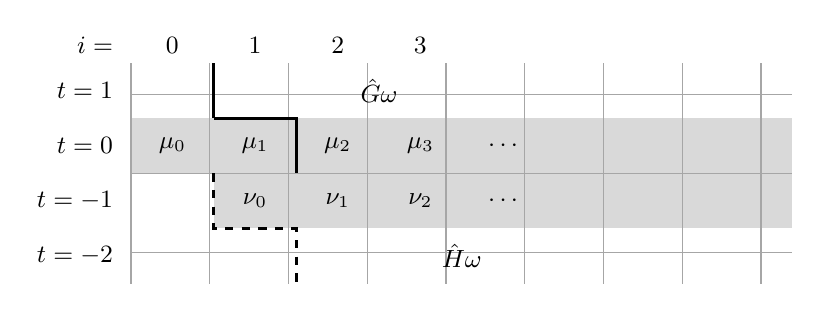
\begin{tikzpicture}[x=1.05cm,y=0.7cm,font=\small]
\foreach \k in {0,...,7} \fill[black!15] (\k-0.5,-0.5) rectangle (\k+0.5,0.5);
\foreach \k in {1,...,7} \fill[black!15] (\k-0.5,-1.5) rectangle (\k+0.5,-0.5);
\draw[black!35,shift={(-0.5,-0.5)}] (0,-2) grid (8,2);
\node at (0,0) {$\mu_0$}; \node at (1,0) {$\mu_1$}; \node at (2,0) {$\mu_2$}; \node at (3,0) {$\mu_3$}; \node at (4,0) {$\cdots$};
\node at (1,-1) {$\nu_0$}; \node at (2,-1) {$\nu_1$}; \node at (3,-1) {$\nu_2$}; \node at (4,-1) {$\cdots$};
\draw[very thick] (0.5,1.5) -- (0.5,0.5);
\draw[very thick] (0.5,0.5) -- (1.5,0.5) -- (1.5,-0.5);
\node at (2.5,1) {$\hat G\omega$};
\draw[very thick,dashed] (0.5,-0.5) -- (0.5,-1.5) -- (1.5,-1.5) -- (1.5,-2.5);
\node at (3.5,-2) {$\hat H\omega$};
\node[left] at (-0.6,1) {$t=1$}; \node[left] at (-0.6,0) {$t=0$}; \node[left] at (-0.6,-1) {$t=-1$}; \node[left] at (-0.6,-2) {$t=-2$};
\foreach \k in {0,1,2,3} \node[above] at (\k,1.5) {$\k$};
\node[above left] at (-0.6,1.5) {$i=$};
\end{tikzpicture}
\caption{The cone code $\omega(Y)$ at the apex $(t,i)=(0,0)$: the entries $\mu_k=Y(0,k)$ and $\nu_k=Y(-1,k+1)$, $k\ge0$ (shaded). The cone codes at the apexes $(0,1)$ and $(0,2)$ are $\sh\omega$ and $\sh^2\omega$. The code $\hat G\omega$ at the apex $(1,1)$ occupies rows $1$ and $0$ (to the right of the solid line), and the code $\hat H\omega$ at the apex $(-1,1)$ occupies rows $-1$ and $-2$ (to the right of the dashed line); both are determined by $\omega$ through \eqref{r30:eq:rec}.}
\label{r30:fig:cone}
\end{figure}

\begin{lemma}\label{r30:lem:I}
\begin{enumerate}
\item For every diagram $Y$,
\[
\omega^{(1,1)}(Y)=\hat G\omega(Y),\quad \omega^{(-1,1)}(Y)=\hat H\omega(Y),\quad \omega^{(0,1)}(Y)=\sh\omega(Y),\quad \omega^{(0,2)}(Y)=\sh^2\omega(Y).
\]
\item For every $\omega\in\A^{\mathbb{N}}$,
\begin{equation}\label{r30:eq:I}
\psi(\hat G\omega)\oplus\psi(\hat H\omega)\oplus\psi(\omega)\oplus\bigl(\psi(\sh\omega)\vee\psi(\sh^2\omega)\bigr)=0.
\end{equation}
\item $\hat G\sh=\sh\hat G$, $\hat H\sh=\sh\hat H$, $\hat GD_1=D_1\hat G$, $\hat HD_1=\hat H$, $\hat HD_2=D_2\hat H$ and $\hat GD_2=\hat G$.
\end{enumerate}
\end{lemma}

\begin{proof}
(1) The last two identities are immediate. By \eqref{r30:eq:rec} at $(0,k+1)$, $Y(1,k+1)=Y(-1,k+1)\oplus Y(0,k)\oplus(Y(0,k+1)\vee Y(0,k+2))=\nu_k\oplus f(\mu_k,\mu_{k+1},\mu_{k+2})$, and $Y(0,k+2)=\mu_{k+2}$; this is $\hat G$. By \eqref{r30:eq:rec} at $(-1,k+2)$, $Y(-2,k+2)=Y(0,k+2)\oplus Y(-1,k+1)\oplus(Y(-1,k+2)\vee Y(-1,k+3))=\mu_{k+2}\oplus f(\nu_k,\nu_{k+1},\nu_{k+2})$, and $Y(-1,k+1)=\nu_k$; this is $\hat H$.

(2) Choose $c$ with $\omega(Y_c)=\omega$. The diagram $Y_{hc}$ satisfies \eqref{r30:eq:rec} at $(0,1)$:
$Y_{hc}(1,1)\oplus Y_{hc}(-1,1)\oplus Y_{hc}(0,0)=Y_{hc}(0,1)\vee Y_{hc}(0,2)$. Now substitute \eqref{r30:eq:psi} and (1).

(3) $\hat G$ and $\hat H$ are given by the same rule at every index $k$, so they commute with $\sh$. The coordinate $\mu_0$ enters $\hat G$ only in the first component of $\hat G(\omega)_0$, through $f(\mu_0,\mu_1,\mu_2)=\mu_0\oplus(\mu_1\vee\mu_2)$, so complementing $\mu_0$ complements the first component of $\hat G(\omega)_0$; this is $\hat GD_1=D_1\hat G$. In that same component $\nu_0\oplus\mu_0$ appears, and $\nu_0$ appears nowhere else in $\hat G$, so $\hat GD_2=\hat G$. The map $\hat H$ does not read $\mu_0$ or $\mu_1$, so $\hat HD_1=\hat H$. Finally, $\nu_0$ enters $\hat H$ only in $\hat H(\omega)_0=(\nu_0,\ \mu_2\oplus\nu_0\oplus(\nu_1\vee\nu_2))$, where complementing it complements both components; this is $\hat HD_2=D_2\hat H$.
\end{proof}

\subsection{Both light edges are permutive}\label{r30:sec:edges}

\begin{proposition}\label{r30:prop:edges}
For every $\omega\in\A^{\mathbb{N}}$, $\psi(D_1\omega)\ne\psi(\omega)$ and $\psi(D_2\omega)\ne\psi(\omega)$.
\end{proposition}

\begin{proof}
Choose $c$ with $\omega(Y_c)=\omega$.

Let $c'$ be $c$ with $y(c_0)$ complemented. Then $\omega(Y_{c'})=D_1\omega$, and $Q=(c,c')$ is a $y$-flip at $0$, with $(U,V)=(0,-2)$ by Lemma~\ref{r30:lem:flips}(2). So $hQ$ has $(U,V)=(0,-2)$. Since $V-U$ is even, Proposition~\ref{r30:prop:profile}(5) gives a middle row at $m=-1$ and $I^+(hQ)=[0,\infty)$, so $\lambda_0(hQ)=0+U=0$. In particular $\Delta_{hQ}(0,0)=1$, that is, $\psi(\omega)\ne\psi(D_1\omega)$.

Let $c'$ be $c$ with $y(c_0)$ and $x(c_1)$ complemented. Then $\omega(Y_{c'})=D_2\omega$, and $Q=(c,c')$ is a $yx$-flip at $0$, so $V(Q)=0$ and $U(Q)\in\{-\infty\}\cup(-\infty,-1]$ (Lemma~\ref{r30:lem:flips}(4)). Then $hQ$ has the same intercepts. If $U(hQ)=-\infty$, then $I^-(hQ)=\Z$ by Proposition~\ref{r30:prop:profile}(3). Otherwise $V-U\ge1$, and by Proposition~\ref{r30:prop:profile}(5) either $I^-(hQ)=(-\infty,t_+-1]$ with $t_+=(V-U+1)/2\ge1$, or $I^-(hQ)=(-\infty,m-1]$ with $m=(V-U)/2\ge1$. In every case $0\in I^-(hQ)$, so $\lambda_0(hQ)=V-0=0$ and $\Delta_{hQ}(0,0)=1$, that is, $\psi(\omega)\ne\psi(D_2\omega)$.
\end{proof}

\begin{corollary}\label{r30:cor:psi}
There is a function $\gamma\colon\A^{\mathbb{N}}\to\{0,1\}$, depending only on the coordinates $0,\dots,R-1$, such that $\psi(\omega)=\mu_0\oplus\gamma(\sh\omega)$ for all $\omega$.
\end{corollary}

\begin{proof}
By Proposition~\ref{r30:prop:edges}, $\psi\oplus\mu_0$ is invariant under $D_1$, so it does not depend on $\mu_0$. It is also invariant under $D_2$, because $D_2$ complements both $\psi$ and $\mu_0$. A function independent of $\mu_0$ and invariant under complementing $(\mu_0,\nu_0)$ is invariant under complementing $\nu_0$. So $\psi\oplus\mu_0$ depends only on $\omega_1,\omega_2,\dots$, and only on $\omega_1,\dots,\omega_R$ because $\psi$ depends only on $\omega_0,\dots,\omega_R$.
\end{proof}

\subsection{The correction term vanishes}\label{r30:sec:gamma}

\begin{lemma}\label{r30:lem:gamma}
Let $\gamma\colon\A^{\mathbb{N}}\to\{0,1\}$ depend on finitely many coordinates, and suppose $\psi(\omega)=\mu_0\oplus\gamma(\sh\omega)$ satisfies \eqref{r30:eq:I}. Then $\gamma\equiv0$.
\end{lemma}

\begin{proof}
For $\theta\in\A^{\mathbb{N}}$ write $\theta_k=(\xi_k,\zeta_k)$. Substitute $\psi$ into \eqref{r30:eq:I} and put $\theta=\sh\omega$, so that $\xi_0=\mu_1(\omega)$ and $\xi_1=\mu_2(\omega)$. Using $\mu_0(\hat G\omega)=\nu_0\oplus\mu_0\oplus(\mu_1\vee\mu_2)$, $\mu_0(\hat H\omega)=\nu_0$, $\sh\hat G=\hat G\sh$ and $\sh\hat H=\hat H\sh$, the terms $\nu_0$ and $\mu_0$ cancel, and \eqref{r30:eq:I} becomes
\begin{equation}\label{r30:eq:star}
\gamma(\hat G\theta)\oplus\gamma(\hat H\theta)\oplus\gamma(\theta)=(\xi_0\vee \xi_1)\oplus\bigl((\xi_0\oplus\gamma(\sh\theta))\vee(\xi_1\oplus\gamma(\sh^2\theta))\bigr).
\end{equation}
This holds for every $\theta\in\A^{\mathbb{N}}$, since $\omega$ is arbitrary.

Three facts are used. (a) $D_1$ and $D_2$ change only $\theta_0$, both complement $\xi_0$, and neither changes $\sh\theta$. (b) The relations of Lemma~\ref{r30:lem:I}(3). (c) Complementing $\xi_0$ while keeping $\xi_1$, $\gamma(\sh\theta)$ and $\gamma(\sh^2\theta)$ fixed changes the right side of \eqref{r30:eq:star} by exactly $\gamma(\sh^2\theta)$. Indeed, $(z\vee e)\oplus(\neg z\vee e)=\neg e$ for bits $z,e$, so the change is $\neg \xi_1\oplus\neg(\xi_1\oplus\gamma(\sh^2\theta))=\gamma(\sh^2\theta)$.

Put $\delta_i=\gamma\oplus(\gamma\circ D_i)$ for $i=1,2$. Evaluate \eqref{r30:eq:star} at $D_1\theta$ and add it to \eqref{r30:eq:star} at $\theta$. By (a)--(c), $\gamma(\hat GD_1\theta)=\gamma(D_1\hat G\theta)$ and $\gamma(\hat HD_1\theta)=\gamma(\hat H\theta)$, so
\begin{equation}\label{r30:eq:one}
\delta_1(\hat G\theta)\oplus\delta_1(\theta)=\gamma(\sh^2\theta).
\end{equation}
In the same way, using $\hat GD_2=\hat G$ and $\hat HD_2=D_2\hat H$,
\begin{equation}\label{r30:eq:two}
\delta_2(\hat H\theta)\oplus\delta_2(\theta)=\gamma(\sh^2\theta).
\end{equation}

Say that a function \emph{depends only on $\theta_0,\dots,\theta_m$} if it takes equal values on sequences that agree in these coordinates; for $m=-1$ this means that it is constant. Let $m\ge-1$ be minimal such that $\gamma$ depends only on $\theta_0,\dots,\theta_m$, and suppose $m\ge0$. Since $D_1$ and $D_2$ act only on $\theta_0$, the functions $\delta_1$ and $\delta_2$ also depend only on $\theta_0,\dots,\theta_m$.

\emph{$\gamma$ does not depend on $\zeta_m$.} For $k\le m$, $\hat G(\theta)_k$ reads only $\xi_k,\xi_{k+1},\xi_{k+2}$ and $\zeta_k$. So the left side of \eqref{r30:eq:one} does not depend on $\zeta_{m+1}$ or $\zeta_{m+2}$, and hence neither does $\gamma(\sh^2\theta)$. Since $(\sh^2\theta)_m=\theta_{m+2}$ and $\sh^2\theta$ ranges over all of $\A^{\mathbb{N}}$, $\gamma$ does not depend on the second component of its coordinate $m$.

\emph{$\gamma$ does not depend on $\xi_m$.} Now $\gamma$, and hence $\delta_2$, depends only on $\theta_0,\dots,\theta_{m-1}$ and $\xi_m$. So $\delta_2(\hat H\theta)$ depends only on $\hat H(\theta)_0,\dots,\hat H(\theta)_{m-1}$ and on the first component of $\hat H(\theta)_m$, which is $\zeta_m$. For $k\le m-1$, $\hat H(\theta)_k$ reads only $\theta_k,\theta_{k+1},\theta_{k+2}$, all with index at most $m+1$. So the left side of \eqref{r30:eq:two} does not depend on $\theta_{m+2}$, and hence neither does $\gamma(\sh^2\theta)$. Since $\gamma(\sh^2\theta)$ depends on $\theta_{m+2}$ only through $\xi_{m+2}$, $\gamma$ does not depend on the first component of its coordinate $m$.

Thus $\gamma$ depends only on $\theta_0,\dots,\theta_{m-1}$, contradicting the minimality of $m$. Hence $m=-1$ and $\gamma$ is constant. Then $\delta_1\equiv0$, and \eqref{r30:eq:one} gives $\gamma(\sh^2\theta)=0$, so $\gamma\equiv0$.
\end{proof}

\subsection{Parity and the proof of Theorem~\ref{thm:rigidity30}}\label{r30:sec:conclusion}

\begin{proposition}\label{r30:prop:trivial}
If $h\in\Aut(X_F)$ satisfies $e^+(h)=e^-(h)=0$, then $h=\mathrm{id}$.
\end{proposition}

\begin{proof}
By Corollary~\ref{r30:cor:psi} and Lemmas~\ref{r30:lem:I}(2) and~\ref{r30:lem:gamma}, $\psi(\omega)=\mu_0$. By \eqref{r30:eq:psi}, $Y_{hc}(t,i)=\mu_0(\omega^{(t,i)}(Y_c))=Y_c(t,i)$ for all $(t,i)$. So $Y_{hc}=Y_c$, and $hc=c$ for every $c$.
\end{proof}

\begin{lemma}\label{r30:lem:parity}
For every $h\in\Aut(X_F)$, $e^+(h)\equiv e^-(h)\pmod 2$.
\end{lemma}

\begin{proof}
For a cell $s\in\A$ let $\bar s=s^{\Z}$ be the constant configuration. Since $f(y,y,y)=y\oplus(y\vee y)=0$, we have $F(\overline{(x,y)})=\overline{(y,x)}$. So $F$ permutes the four constant configurations as the transposition exchanging $\overline{(0,1)}$ and $\overline{(1,0)}$, fixing the other two. Every $h\in\Aut(X_F)$ commutes with $\sh$, so it maps the four $\sh$-fixed points bijectively to themselves, and the induced permutation commutes with that of $F$. The centralizer in $\Sym(4)$ of a transposition $(\alpha\,\beta)$ is $\langle(\alpha\,\beta)\rangle\times\langle(\alpha'\,\beta')\rangle$, where $\{\alpha',\beta'\}$ is the complement of $\{\alpha,\beta\}$. Every element of this group has order at most $2$, so $h^2$ fixes every constant configuration.

Suppose $e^+(h)+e^-(h)$ is odd. Put $a=-(e^+(h)+e^-(h)+1)/2$ and $b=(e^+(h)-e^-(h)-1)/2$, which are integers. By Corollary~\ref{r30:cor:offsets}, $(e^+,e^-)(\sh^aF^b)=(b-a,-a-b)=(e^+(h),e^-(h)+1)$, so $h_1=F^{-b}\sh^{-a}h$ has offsets $(0,-1)$. Then $h_1^2$ has offsets $(0,-2)=(e^+,e^-)(\sh F)$, so $h_1^2(\sh F)^{-1}$ has offsets $(0,0)$, and $h_1^2=\sh F$ by Proposition~\ref{r30:prop:trivial}. But $h_1^2$ fixes every constant configuration, while $\sh F$ exchanges $\overline{(0,1)}$ and $\overline{(1,0)}$. This is a contradiction.
\end{proof}

\begin{proof}[Proof of Theorem~\ref{thm:rigidity30}]
Let $h\in\Aut(X_F)$. By Lemma~\ref{r30:lem:parity}, $e^+(h)+e^-(h)$ is even, so $a=-\tfrac12(e^+(h)+e^-(h))$ and $b=\tfrac12(e^+(h)-e^-(h))$ are integers, and $(e^+,e^-)(\sh^aF^b)=(b-a,-a-b)=(e^+(h),e^-(h))$. Hence $h_0=F^{-b}\sh^{-a}h$ has $e^+(h_0)=e^-(h_0)=0$, so $h_0=\mathrm{id}$ by Proposition~\ref{r30:prop:trivial}, and $h=\sh^aF^b$. Uniqueness of $(a,b)$ and $\langle\sh,F\rangle\cong\Z^2$ are Corollary~\ref{r30:cor:offsets}(4). By Lemma~\ref{lem:spacetime}, this describes $\Aut(X_{F_{30}})$.
\end{proof}

\begin{remark}
The properties of rule $30$ used are the following: the second-order rule is permutive in the previous row and in the left neighbour, so it satisfies Lemma~\ref{r30:lem:R}; the maximum principle (Lemma~\ref{r30:lem:max}), which uses only Lemmas~\ref{r30:lem:onset} and~\ref{r30:lem:flips}; the strong connectivity of the light-speed window graph $\Lambda_M$ (Lemma~\ref{r30:lem:lambda}), whose proof uses the specific form $a\oplus(b\vee c)$ only through the stationary loop \eqref{r30:eq:loop}; the cone identity \eqref{r30:eq:I} forces the correction to vanish (Lemma~\ref{r30:lem:gamma}); and $f(y,y,y)=0$, which is used for the parity. Permutivity in the right argument, which rule $30$ lacks, is never used.
\end{remark}
